% Options for packages loaded elsewhere
\PassOptionsToPackage{unicode}{hyperref}
\PassOptionsToPackage{hyphens}{url}
\PassOptionsToPackage{dvipsnames,svgnames,x11names}{xcolor}
\documentclass[
  10pt,
]{article}
\usepackage{xcolor}
\usepackage{amsmath,amssymb}
\setcounter{secnumdepth}{-\maxdimen} % remove section numbering
\usepackage{iftex}
\ifPDFTeX
  \usepackage[T1]{fontenc}
  \usepackage[utf8]{inputenc}
  \usepackage{textcomp} % provide euro and other symbols
\else % if luatex or xetex
  \usepackage{unicode-math} % this also loads fontspec
  \defaultfontfeatures{Scale=MatchLowercase}
  \defaultfontfeatures[\rmfamily]{Ligatures=TeX,Scale=1}
\fi
\usepackage{lmodern}
\ifPDFTeX\else
  % xetex/luatex font selection
\fi
% Use upquote if available, for straight quotes in verbatim environments
\IfFileExists{upquote.sty}{\usepackage{upquote}}{}
\IfFileExists{microtype.sty}{% use microtype if available
  \usepackage[]{microtype}
  \UseMicrotypeSet[protrusion]{basicmath} % disable protrusion for tt fonts
}{}
\makeatletter
\@ifundefined{KOMAClassName}{% if non-KOMA class
  \IfFileExists{parskip.sty}{%
    \usepackage{parskip}
  }{% else
    \setlength{\parindent}{0pt}
    \setlength{\parskip}{6pt plus 2pt minus 1pt}}
}{% if KOMA class
  \KOMAoptions{parskip=half}}
\makeatother
\usepackage{longtable,booktabs,array}
\usepackage{caption}
\captionsetup[table]{skip=6pt}
\newcounter{none} % for unnumbered tables
\usepackage{calc} % for calculating minipage widths
% Correct order of tables after \paragraph or \subparagraph
\usepackage{etoolbox}
\makeatletter
\patchcmd\longtable{\par}{\if@noskipsec\mbox{}\fi\par}{}{}
\makeatother
% Allow footnotes in longtable head/foot
\IfFileExists{footnotehyper.sty}{\usepackage{footnotehyper}}{\usepackage{footnote}}
\makesavenoteenv{longtable}
\usepackage{graphicx}
\makeatletter
\newsavebox\pandoc@box
\newcommand*\pandocbounded[1]{% scales image to fit in text height/width
  \sbox\pandoc@box{#1}%
  \Gscale@div\@tempa{\textheight}{\dimexpr\ht\pandoc@box+\dp\pandoc@box\relax}%
  \Gscale@div\@tempb{\linewidth}{\wd\pandoc@box}%
  \ifdim\@tempb\p@<\@tempa\p@\let\@tempa\@tempb\fi% select the smaller of both
  \ifdim\@tempa\p@<\p@\scalebox{\@tempa}{\usebox\pandoc@box}%
  \else\usebox{\pandoc@box}%
  \fi%
}
% Set default figure placement to htbp
\def\fps@figure{htbp}
\makeatother
\setlength{\emergencystretch}{3em} % prevent overfull lines
\providecommand{\tightlist}{%
  \setlength{\itemsep}{0pt}\setlength{\parskip}{0pt}}
\usepackage[letterpaper,margin=0.8in]{geometry}
\usepackage{booktabs,longtable,array}
\let\oldlongtable\longtable
\def\longtable{\footnotesize\oldlongtable}
\setlength{\tabcolsep}{4pt}
\setlength{\parindent}{0pt}
\setlength{\parskip}{5pt}
\setlength{\emergencystretch}{3em}
\usepackage{bookmark}
\IfFileExists{xurl.sty}{\usepackage{xurl}}{} % add URL line breaks if available
\urlstyle{same}
% fallback for those not using the hyperref driver hyperxmp:
\makeatletter
\@ifundefined{xmpquote}{\newcommand{\xmpquote}[1]{#1}}{}
\makeatother
\hypersetup{
  pdftitle={Structured masking and PC loss: metrics by parameter},
  colorlinks=true,
  linkcolor={Maroon},
  filecolor={Maroon},
  citecolor={Blue},
  urlcolor={Blue},
  pdfcreator={LaTeX via pandoc}}

\title{Structured masking and PC loss: metrics by parameter}
\author{}
\date{}

\begin{document}
\maketitle

\textbf{Setup (all tables).} 4M base, 3 000 train plants (1 view / plant
/ epoch), global batch 32, same input corruption in every run
(procedural Bézier leaves + sensor noise). Validation: fixed 225-view
subset, \textbf{completely clean} (no leaves, no noise), uniform token
mask (no blobs), scored against the clean sample. \textbf{mean ±
half-range over seeds} where 2 seeds. Seed-to-seed noise floor (same
config twice): F1@0.03 0.3 \%, F1@0.01 1.7 \%, Chamfer 0.6 \%.
F1@\(\tau\), recall, precision: fraction of points within \(\tau\);
Chamfer and MSE: lower is better.

\section{1. Structured masking --- 600 epochs, 2
seeds}\label{structured-masking-600-epochs-2-seeds}

{\def\LTcaptype{none} % do not increment counter
\begin{longtable}[]{@{}
  >{\raggedright\arraybackslash}p{(\linewidth - 16\tabcolsep) * \real{0.1111}}
  >{\raggedright\arraybackslash}p{(\linewidth - 16\tabcolsep) * \real{0.1111}}
  >{\raggedright\arraybackslash}p{(\linewidth - 16\tabcolsep) * \real{0.1111}}
  >{\raggedright\arraybackslash}p{(\linewidth - 16\tabcolsep) * \real{0.1111}}
  >{\raggedright\arraybackslash}p{(\linewidth - 16\tabcolsep) * \real{0.1111}}
  >{\raggedright\arraybackslash}p{(\linewidth - 16\tabcolsep) * \real{0.1111}}
  >{\raggedright\arraybackslash}p{(\linewidth - 16\tabcolsep) * \real{0.1111}}
  >{\raggedright\arraybackslash}p{(\linewidth - 16\tabcolsep) * \real{0.1111}}
  >{\raggedright\arraybackslash}p{(\linewidth - 16\tabcolsep) * \real{0.1111}}@{}}
\toprule\noalign{}
\begin{minipage}[b]{\linewidth}\raggedright
structured
\end{minipage} & \begin{minipage}[b]{\linewidth}\raggedright
blob size
\end{minipage} & \begin{minipage}[b]{\linewidth}\raggedright
edge bias
\end{minipage} & \begin{minipage}[b]{\linewidth}\raggedright
F1@0.03
\end{minipage} & \begin{minipage}[b]{\linewidth}\raggedright
F1@0.01
\end{minipage} & \begin{minipage}[b]{\linewidth}\raggedright
recall@0.03
\end{minipage} & \begin{minipage}[b]{\linewidth}\raggedright
precision@0.03
\end{minipage} & \begin{minipage}[b]{\linewidth}\raggedright
Chamfer \(\times10^{-3}\)
\end{minipage} & \begin{minipage}[b]{\linewidth}\raggedright
Depth MSE \(\times10^{-2}\)
\end{minipage} \\
\midrule\noalign{}
\endhead
\bottomrule\noalign{}
\endlastfoot
off & -- & -- & \textbf{0.788 ± 0.054} & \textbf{0.291 ± 0.061} &
\textbf{0.712 ± 0.062} & \textbf{0.904 ± 0.038} & \textbf{2.20 ± 0.39} &
4.48 ± 0.22 \\
on & 0.02 (no blobs) & 1.5 & 0.633 ± 0.022 & 0.195 ± 0.011 & 0.513 ±
0.028 & 0.849 ± 0.001 & 3.90 ± 0.32 & \textbf{3.82 ± 0.02} \\
on & 0.20 & 0 & 0.643 ± 0.030 & 0.189 ± 0.009 & 0.529 ± 0.042 & 0.845 ±
0.003 & 3.77 ± 0.45 & 4.00 ± 0.06 \\
on & 0.20 & 1.5 & 0.605 ± 0.003 & 0.176 ± 0.001 & 0.478 ± 0.003 & 0.848
± 0.003 & 4.36 ± 0.01 & 3.88 ± 0.03 \\
\end{longtable}
}

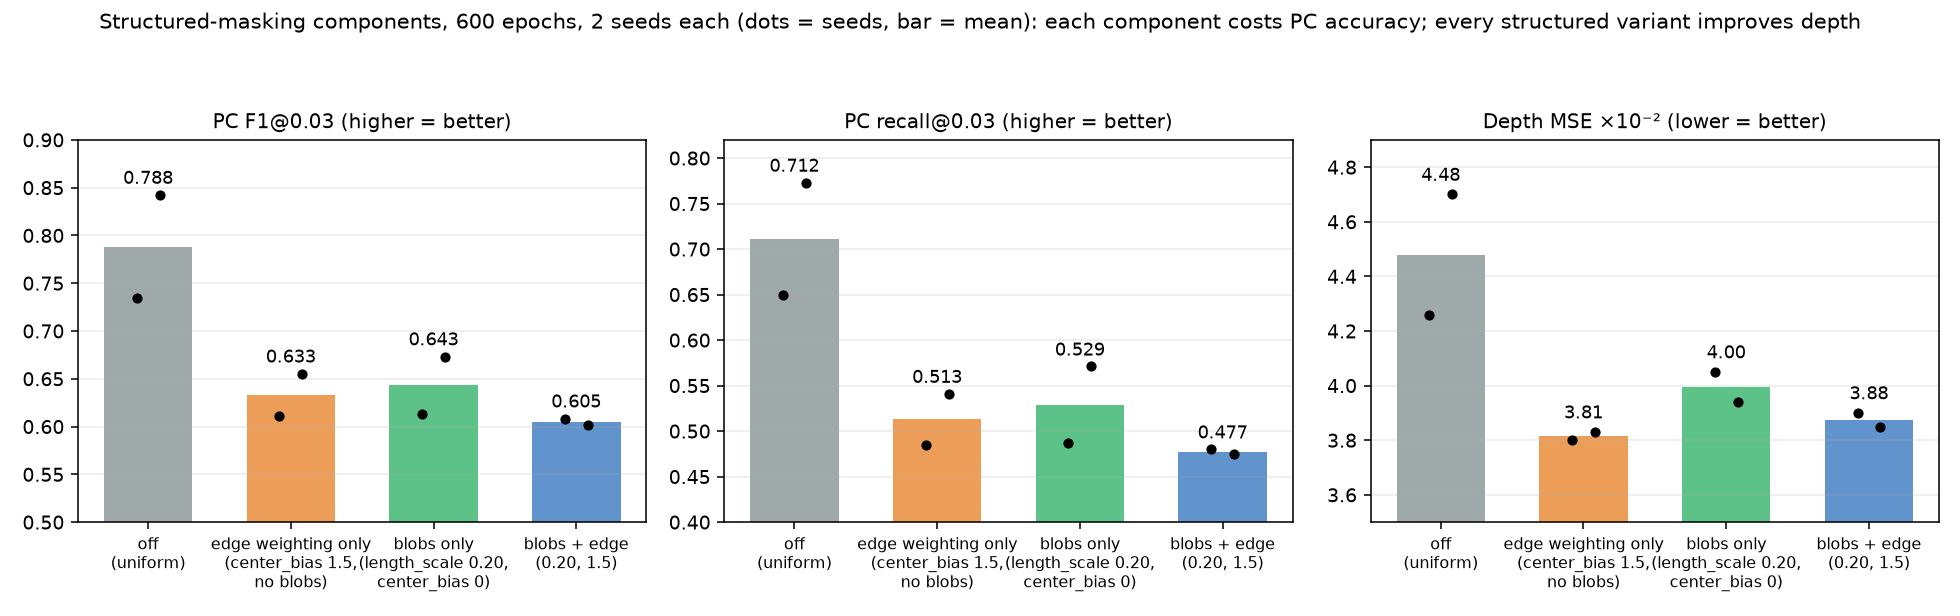
\includegraphics[width=1\linewidth,height=\textheight,keepaspectratio]{structured_mask_components.png}

\textbf{How a structured mask is made.} Each patch gets a score =
\emph{random cosine field} + \texttt{center\_bias} \(\times\) radius;
the 49 lowest-scoring patches stay visible, the other 147 are hidden.
The cosine field is a smooth random surface, redrawn every sample (its
smoothness sets the blob size, \texttt{length\_scale}); the edge term
tilts it toward the border. The field has standard deviation 1 and the
edge term spans 0--1.5 at \texttt{center\_bias} 1.5, so \textbf{neither
dominates}: blobs still land anywhere, and the border is favoured only
on average. That is why the masks look mixed rather than edge-only.

{\def\LTcaptype{none} % do not increment counter
\begin{longtable}[]{@{}
  >{\raggedright\arraybackslash}p{(\linewidth - 6\tabcolsep) * \real{0.2500}}
  >{\raggedright\arraybackslash}p{(\linewidth - 6\tabcolsep) * \real{0.2500}}
  >{\raggedright\arraybackslash}p{(\linewidth - 6\tabcolsep) * \real{0.2500}}
  >{\raggedright\arraybackslash}p{(\linewidth - 6\tabcolsep) * \real{0.2500}}@{}}
\toprule\noalign{}
\begin{minipage}[b]{\linewidth}\raggedright
\texttt{center\_bias}
\end{minipage} & \begin{minipage}[b]{\linewidth}\raggedright
P(masked), centre
\end{minipage} & \begin{minipage}[b]{\linewidth}\raggedright
P(masked), corner
\end{minipage} & \begin{minipage}[b]{\linewidth}\raggedright
resulting mask
\end{minipage} \\
\midrule\noalign{}
\endhead
\bottomrule\noalign{}
\endlastfoot
0 & 0.75 & 0.75 & blobs anywhere \\
\textbf{1.5 (used)} & 0.53 & 0.89 & blobs anywhere, leaning to the
border \\
5 & 0.13 & 0.99 & a near-fixed border ring, centre visible \\
\end{longtable}
}

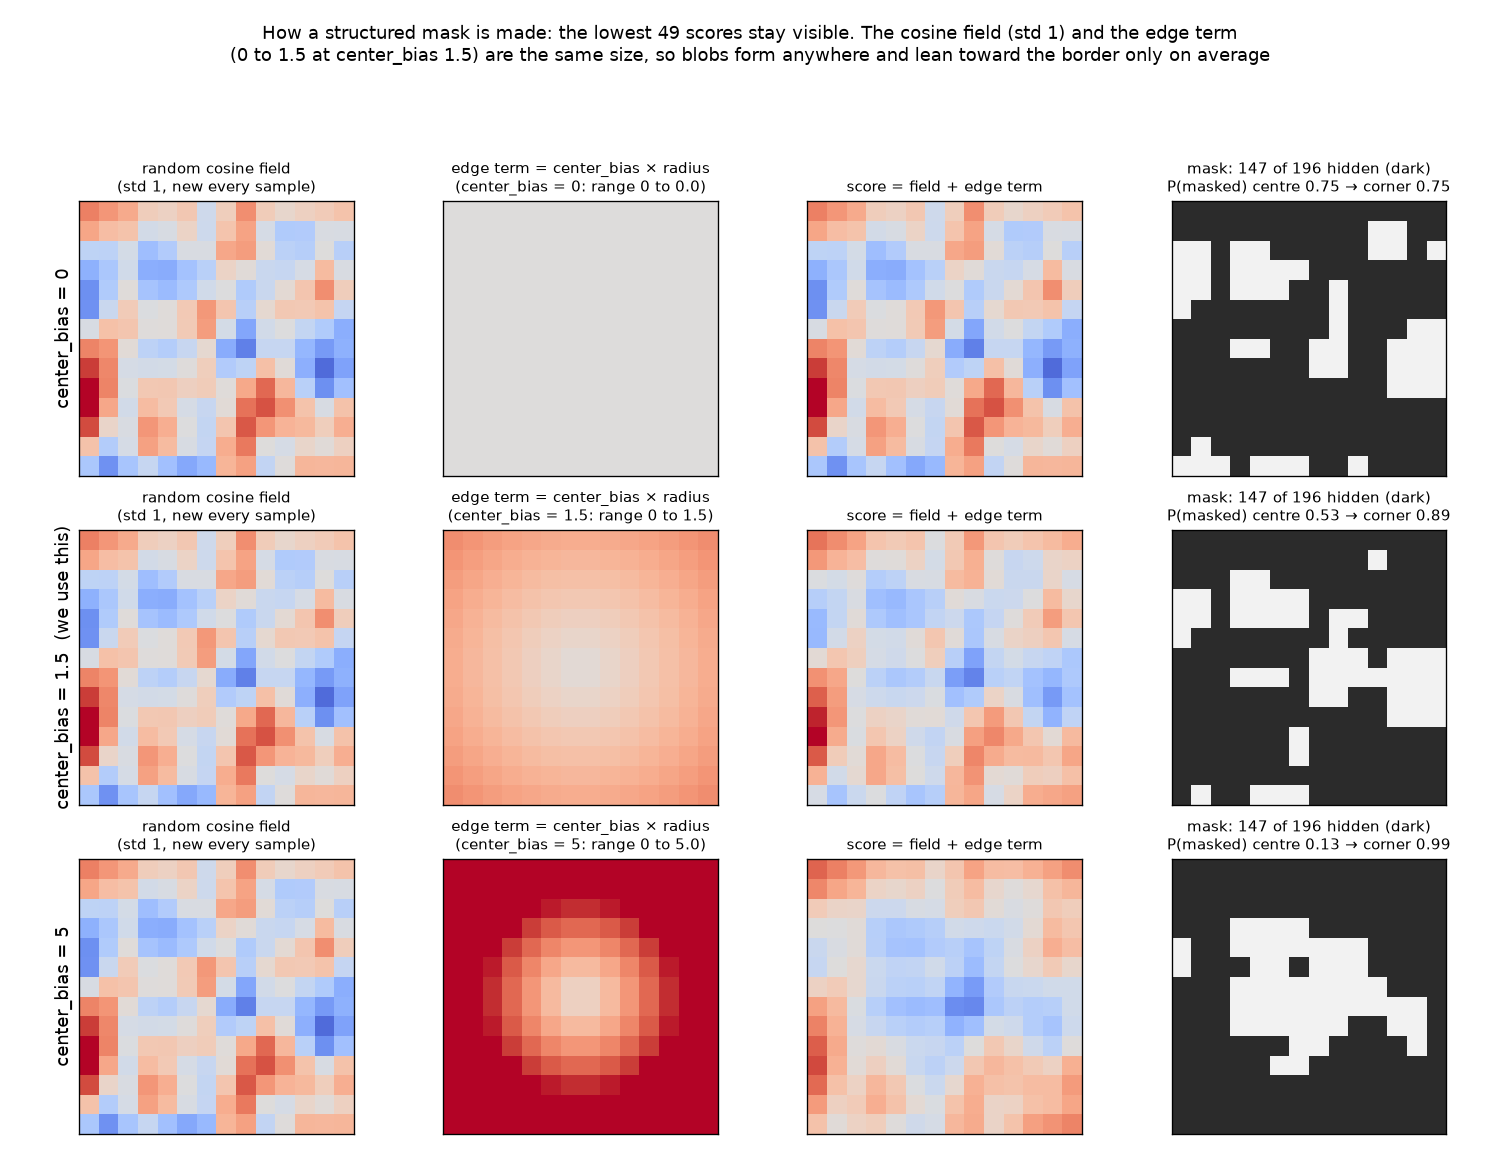
\includegraphics[width=0.92\linewidth,height=\textheight,keepaspectratio]{mask_field_vs_bias.png}

The occluding leaves (section 6) are a separate mechanism acting on the
\emph{input pixels and points}, not on the token mask. They are also not
edge-only by design: each leaf is rooted just outside the frame but
grows 0.6--1.2 image units inward, so leaf coverage is highest mid-way
out (about 47 \% of pixels at radius 0.5) and about 5 \% at the centre.

\section{2. Blob size and sensor noise --- 30k steps (320 epochs), 1
seed}\label{blob-size-and-sensor-noise-30k-steps-320-epochs-1-seed}

{\def\LTcaptype{none} % do not increment counter
\begin{longtable}[]{@{}
  >{\raggedright\arraybackslash}p{(\linewidth - 12\tabcolsep) * \real{0.1429}}
  >{\raggedright\arraybackslash}p{(\linewidth - 12\tabcolsep) * \real{0.1429}}
  >{\raggedright\arraybackslash}p{(\linewidth - 12\tabcolsep) * \real{0.1429}}
  >{\raggedright\arraybackslash}p{(\linewidth - 12\tabcolsep) * \real{0.1429}}
  >{\raggedright\arraybackslash}p{(\linewidth - 12\tabcolsep) * \real{0.1429}}
  >{\raggedright\arraybackslash}p{(\linewidth - 12\tabcolsep) * \real{0.1429}}
  >{\raggedright\arraybackslash}p{(\linewidth - 12\tabcolsep) * \real{0.1429}}@{}}
\toprule\noalign{}
\begin{minipage}[b]{\linewidth}\raggedright
blob size
\end{minipage} & \begin{minipage}[b]{\linewidth}\raggedright
sensor noise
\end{minipage} & \begin{minipage}[b]{\linewidth}\raggedright
F1@0.03
\end{minipage} & \begin{minipage}[b]{\linewidth}\raggedright
F1@0.01
\end{minipage} & \begin{minipage}[b]{\linewidth}\raggedright
Chamfer \(\times10^{-3}\)
\end{minipage} & \begin{minipage}[b]{\linewidth}\raggedright
RGB MSE
\end{minipage} & \begin{minipage}[b]{\linewidth}\raggedright
Depth MSE \(\times10^{-2}\)
\end{minipage} \\
\midrule\noalign{}
\endhead
\bottomrule\noalign{}
\endlastfoot
0.35 & 1× & 0.583 & 0.158 & 4.70 & 0.674 & 3.35 \\
0.20 & 1× & 0.586 & 0.157 & 4.64 & 0.665 & 3.36 \\
0.20 & 0.5× & 0.582 & 0.154 & 4.72 & 0.672 & 3.22 \\
0.20 & 2× & 0.582 & 0.150 & 4.68 & 0.661 & 3.22 \\
0.20 & 1× (repeat, seed 1) & 0.584 & 0.154 & 4.67 & 0.677 & 3.00 \\
\end{longtable}
}

Blob size = \texttt{length\_scale} (0.20 about 10 \%, 0.35 about 18 \%
of the frame width; 0.02 = no blobs). Edge bias = \texttt{center\_bias},
push toward the frame border (at 1.5: P(masked) 0.64 at the centre, 0.89
at the corners). Sensor noise 1× = pixels ±0.03, depth ±1.5 \%, points
±0.008. Mask ratio 75 \% in every row.

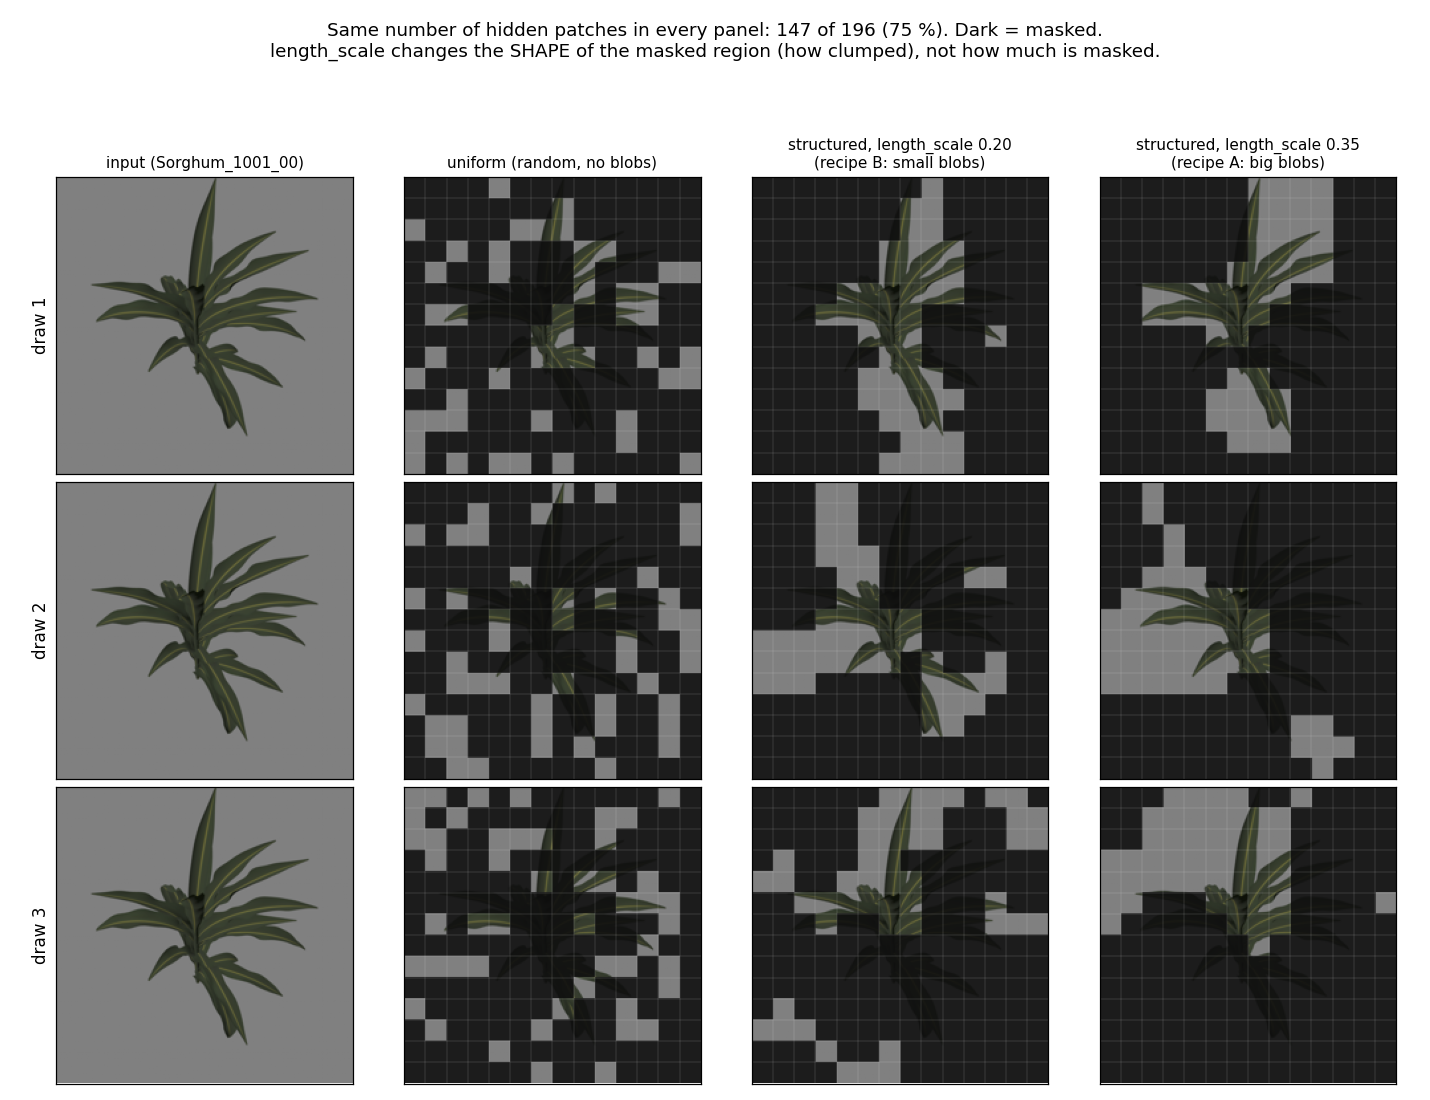
\includegraphics[width=0.85\linewidth,height=\textheight,keepaspectratio]{mask_blob_size.png}

\emph{Training token masks on one image (illustration, not a validation
result). Validation never uses blobs: its token mask is always the
uniform one (2nd column).}

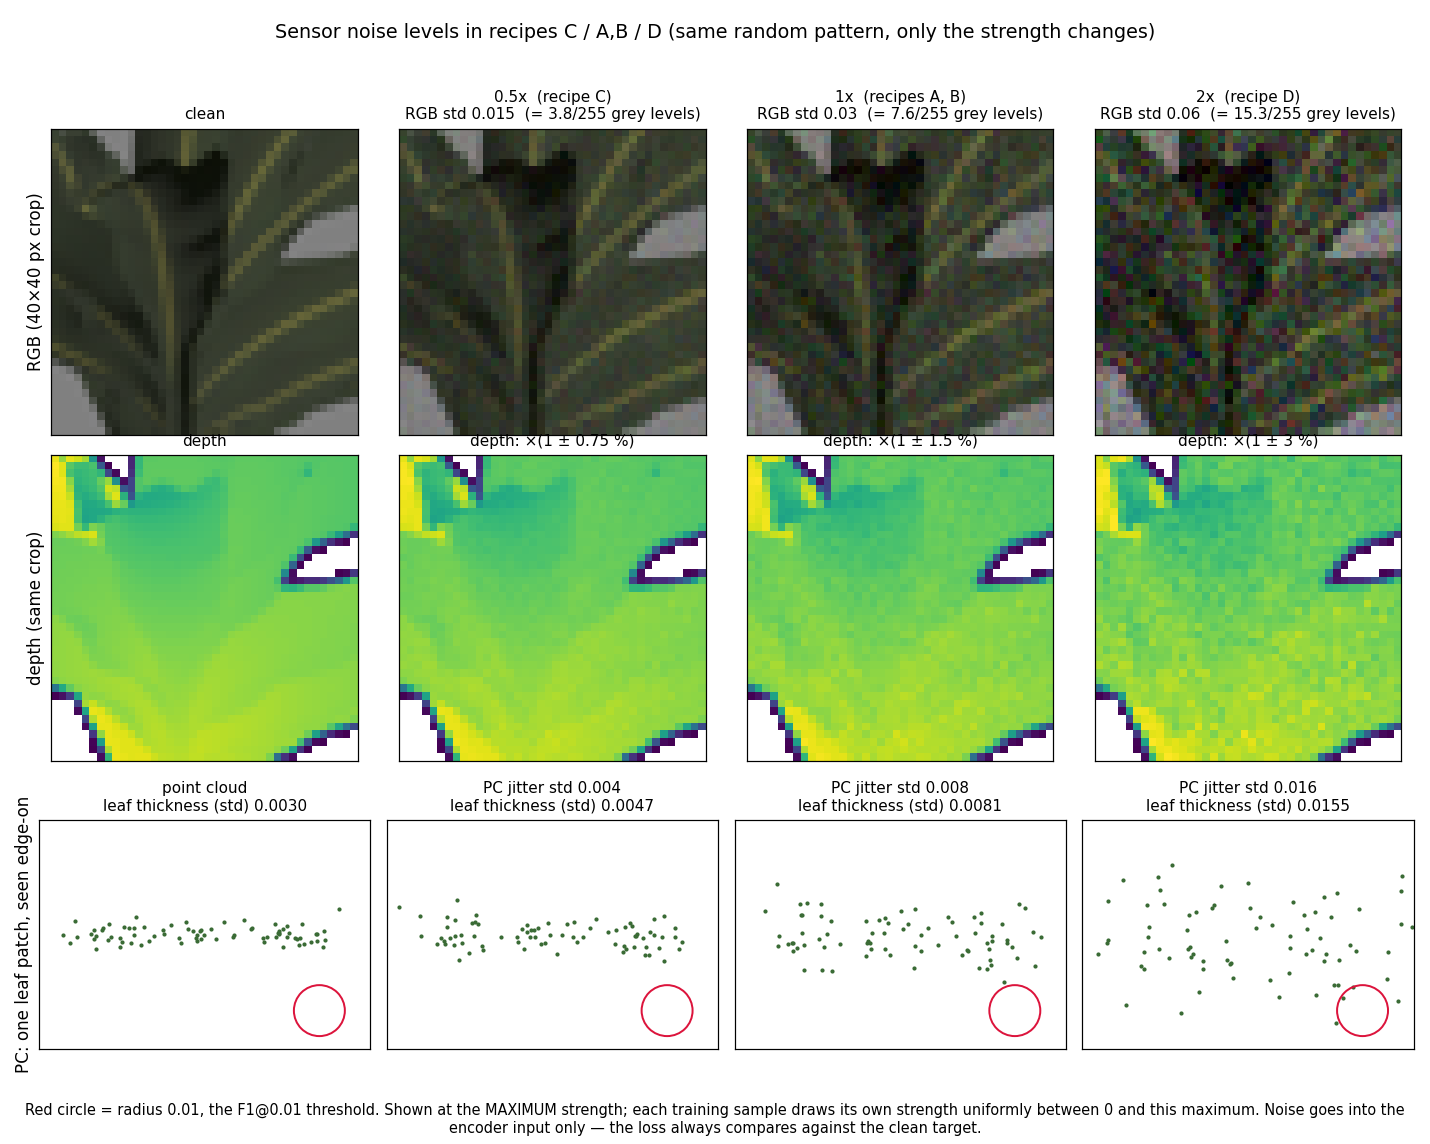
\includegraphics[width=0.85\linewidth,height=\textheight,keepaspectratio]{noise_levels.png}

\newpage

\section{3. Point-cloud loss --- 600 epochs, 1 seed (masking: 0.20 /
1.5)}\label{point-cloud-loss-600-epochs-1-seed-masking-0.20-1.5}

{\def\LTcaptype{none} % do not increment counter
\begin{longtable}[]{@{}
  >{\raggedright\arraybackslash}p{(\linewidth - 14\tabcolsep) * \real{0.1250}}
  >{\raggedright\arraybackslash}p{(\linewidth - 14\tabcolsep) * \real{0.1250}}
  >{\raggedright\arraybackslash}p{(\linewidth - 14\tabcolsep) * \real{0.1250}}
  >{\raggedright\arraybackslash}p{(\linewidth - 14\tabcolsep) * \real{0.1250}}
  >{\raggedright\arraybackslash}p{(\linewidth - 14\tabcolsep) * \real{0.1250}}
  >{\raggedright\arraybackslash}p{(\linewidth - 14\tabcolsep) * \real{0.1250}}
  >{\raggedright\arraybackslash}p{(\linewidth - 14\tabcolsep) * \real{0.1250}}
  >{\raggedright\arraybackslash}p{(\linewidth - 14\tabcolsep) * \real{0.1250}}@{}}
\toprule\noalign{}
\begin{minipage}[b]{\linewidth}\raggedright
loss
\end{minipage} & \begin{minipage}[b]{\linewidth}\raggedright
setting
\end{minipage} & \begin{minipage}[b]{\linewidth}\raggedright
F1@0.03
\end{minipage} & \begin{minipage}[b]{\linewidth}\raggedright
F1@0.01
\end{minipage} & \begin{minipage}[b]{\linewidth}\raggedright
recall@0.03
\end{minipage} & \begin{minipage}[b]{\linewidth}\raggedright
precision@0.03
\end{minipage} & \begin{minipage}[b]{\linewidth}\raggedright
Chamfer \(\times10^{-3}\)
\end{minipage} & \begin{minipage}[b]{\linewidth}\raggedright
Depth MSE \(\times10^{-2}\)
\end{minipage} \\
\midrule\noalign{}
\endhead
\bottomrule\noalign{}
\endlastfoot
QAL & \(\tau\) = 0.01, \(\alpha\) = 100 & \textbf{0.608} &
\textbf{0.176} & 0.480 & \textbf{0.850} & 4.35 & 3.90 \\
Chamfer (squared) & weight 10 & 0.578 & 0.144 & 0.450 & 0.846 & 4.35 &
\textbf{3.63} \\
Sinkhorn only & blur 0.02, 2 048 pts & 0.474 & 0.136 & \textbf{0.710} &
0.359 & 10.32 & 4.07 \\
\end{longtable}
}

\section{\texorpdfstring{4. QAL \(\tau\) and \(\alpha\) --- 30k steps
(320 epochs), 1
seed}{4. QAL \textbackslash tau and \textbackslash alpha --- 30k steps (320 epochs), 1 seed}}\label{qal-tau-and-alpha-30k-steps-320-epochs-1-seed}

{\def\LTcaptype{none} % do not increment counter
\begin{longtable}[]{@{}
  >{\raggedright\arraybackslash}p{(\linewidth - 14\tabcolsep) * \real{0.1250}}
  >{\raggedright\arraybackslash}p{(\linewidth - 14\tabcolsep) * \real{0.1250}}
  >{\raggedright\arraybackslash}p{(\linewidth - 14\tabcolsep) * \real{0.1250}}
  >{\raggedright\arraybackslash}p{(\linewidth - 14\tabcolsep) * \real{0.1250}}
  >{\raggedright\arraybackslash}p{(\linewidth - 14\tabcolsep) * \real{0.1250}}
  >{\raggedright\arraybackslash}p{(\linewidth - 14\tabcolsep) * \real{0.1250}}
  >{\raggedright\arraybackslash}p{(\linewidth - 14\tabcolsep) * \real{0.1250}}
  >{\raggedright\arraybackslash}p{(\linewidth - 14\tabcolsep) * \real{0.1250}}@{}}
\toprule\noalign{}
\begin{minipage}[b]{\linewidth}\raggedright
loss
\end{minipage} & \begin{minipage}[b]{\linewidth}\raggedright
\(\tau\)
\end{minipage} & \begin{minipage}[b]{\linewidth}\raggedright
\(\alpha\)
\end{minipage} & \begin{minipage}[b]{\linewidth}\raggedright
F1@0.03
\end{minipage} & \begin{minipage}[b]{\linewidth}\raggedright
F1@0.01
\end{minipage} & \begin{minipage}[b]{\linewidth}\raggedright
recall@0.03
\end{minipage} & \begin{minipage}[b]{\linewidth}\raggedright
precision@0.03
\end{minipage} & \begin{minipage}[b]{\linewidth}\raggedright
Chamfer \(\times10^{-3}\)
\end{minipage} \\
\midrule\noalign{}
\endhead
\bottomrule\noalign{}
\endlastfoot
QAL & 0.005 & 100 & 0.582 & 0.154 & 0.460 & 0.822 & 4.70 \\
QAL & \textbf{0.01} & \textbf{100} & \textbf{0.584} & \textbf{0.154} &
0.465 & 0.818 & \textbf{4.67} \\
QAL & 0.02 & 100 & 0.585 & 0.139 & 0.469 & 0.813 & 4.74 \\
QAL & 0.01 & 30 & 0.576 & 0.147 & 0.453 & 0.824 & 4.71 \\
QAL & 0.01 & 300 & 0.580 & 0.163 & 0.461 & 0.818 & 4.66 \\
Chamfer (squared) & -- & weight 3 & 0.550 & 0.126 & 0.428 & 0.820 &
4.72 \\
\end{longtable}
}

\section{5. Params encoding --- 600 epochs, 2 seeds (masking: 0.20 /
1.5,
QAL)}\label{params-encoding-600-epochs-2-seeds-masking-0.20-1.5-qal}

{\def\LTcaptype{none} % do not increment counter
\begin{longtable}[]{@{}
  >{\raggedright\arraybackslash}p{(\linewidth - 8\tabcolsep) * \real{0.2000}}
  >{\raggedright\arraybackslash}p{(\linewidth - 8\tabcolsep) * \real{0.2000}}
  >{\raggedright\arraybackslash}p{(\linewidth - 8\tabcolsep) * \real{0.2000}}
  >{\raggedright\arraybackslash}p{(\linewidth - 8\tabcolsep) * \real{0.2000}}
  >{\raggedright\arraybackslash}p{(\linewidth - 8\tabcolsep) * \real{0.2000}}@{}}
\toprule\noalign{}
\begin{minipage}[b]{\linewidth}\raggedright
params
\end{minipage} & \begin{minipage}[b]{\linewidth}\raggedright
F1@0.03
\end{minipage} & \begin{minipage}[b]{\linewidth}\raggedright
F1@0.01
\end{minipage} & \begin{minipage}[b]{\linewidth}\raggedright
recall@0.03
\end{minipage} & \begin{minipage}[b]{\linewidth}\raggedright
Chamfer \(\times10^{-3}\)
\end{minipage} \\
\midrule\noalign{}
\endhead
\bottomrule\noalign{}
\endlastfoot
v1 (original) & 0.605 ± 0.003 & 0.176 ± 0.001 & 0.478 ± 0.003 & 4.36 ±
0.01 \\
v2 + camera pose / scale (spline weight 0.6) & \textbf{0.617 ± 0.002} &
\textbf{0.220 ± 0.005} & 0.483 ± 0.000 & \textbf{4.28 ± 0.08} \\
\end{longtable}
}

\textbf{What v1 got wrong, measured on the data, and what v2 changes:}

{\def\LTcaptype{none} % do not increment counter
\begin{longtable}[]{@{}
  >{\raggedright\arraybackslash}p{(\linewidth - 2\tabcolsep) * \real{0.6176}}
  >{\raggedright\arraybackslash}p{(\linewidth - 2\tabcolsep) * \real{0.3824}}@{}}
\toprule\noalign{}
\begin{minipage}[b]{\linewidth}\raggedright
v1 problem
\end{minipage} & \begin{minipage}[b]{\linewidth}\raggedright
v2 change
\end{minipage} \\
\midrule\noalign{}
\endhead
\bottomrule\noalign{}
\endlastfoot
The params describe the plant in its \textbf{world frame}, but the
target point cloud is in the \textbf{camera frame}
(\texttt{*\_nc\_cam.ply} = worldToCamera \(\times\) world). The camera
pose that links the two (\texttt{camera\_pose.json}) was never read, so
the model had to guess the viewpoint from the images. & camera rotation
given to the model as an always-visible token (the translation needs
none: centring the cloud removes it) \\
Each point cloud is rescaled to unit radius, which erases plant size:
corr(stem length, cloud height) is 0.68 before rescaling, 0.08 after. &
the rescaling radius added to the same token \\
5 of the 9 plant values (\texttt{panicle\_*}) are constant in the data;
angles wrap around at 360°. & constants dropped, angles as sin/cos, all
values z-scored, leaf count added \\
z-scored targets are about 6\(\times\) larger than v1's {[}0, 1{]}
values, so at the same loss weight the param loss takes gradient from
the point-cloud loss. & spline loss weight 5 \(\to\) 0.6 \\
\end{longtable}
}

\textbf{How we know the frames} --- files in every sample folder,
checked on plant Sorghum\_7 (all 10 views):

{\def\LTcaptype{none} % do not increment counter
\begin{longtable}[]{@{}
  >{\raggedright\arraybackslash}p{(\linewidth - 2\tabcolsep) * \real{0.4167}}
  >{\raggedright\arraybackslash}p{(\linewidth - 2\tabcolsep) * \real{0.5833}}@{}}
\toprule\noalign{}
\begin{minipage}[b]{\linewidth}\raggedright
check
\end{minipage} & \begin{minipage}[b]{\linewidth}\raggedright
result
\end{minipage} \\
\midrule\noalign{}
\endhead
\bottomrule\noalign{}
\endlastfoot
training target \texttt{Sorghum\_7\_nc\_cam.ply} vs the world cloud
\texttt{Sorghum\_7\_nc.ply} & worldToCamera (from
\texttt{camera\_pose.json}) \(\times\) world cloud = target cloud, point
by point, error 0 (72 261 points); without the transform they differ by
up to 2.9--3.8 \\
which files change with the view & \texttt{\_nc.ply} and
\texttt{\_spline.yml} (the params) are byte-identical in all 10 view
folders; \texttt{\_nc\_cam.ply} and \texttt{camera\_pose.json} differ in
every view \\
params: \texttt{stem\_direction} & {[}0.04, 1.00, -0.02{]} = world up
(+y), the same in every view; the same stem in camera coordinates points
24--133° apart across the 10 views \\
params: leaf \texttt{Center\ Points} (3 648 points) & lie on the world
cloud (median distance 0.004); median 1.7 from the camera cloud as
stored \\
what the v1 loader reads & \texttt{*\_nc\_cam.ply} as target and input,
the params YAML as is; \texttt{camera\_pose.json} is never opened \\
\end{longtable}
}

Result: F1@0.01 +25 \% (0.176 \(\to\) 0.220, seed spread \(\leq\)
0.005), i.e.~points are placed more precisely. The four changes were
made together, so this does not say how much comes from the camera token
alone. The params already helped in v1: replacing each sample's own
params with the validation mean made its Chamfer 7 \% worse (same masks,
30k-step model).

\newpage

\section{6. Input corruption (fixed in every run): procedural Bézier
leaves}\label{input-corruption-fixed-in-every-run-procedural-buxe9zier-leaves}

{\def\LTcaptype{none} % do not increment counter
\begin{longtable}[]{@{}
  >{\raggedright\arraybackslash}p{(\linewidth - 12\tabcolsep) * \real{0.1429}}
  >{\raggedright\arraybackslash}p{(\linewidth - 12\tabcolsep) * \real{0.1429}}
  >{\raggedright\arraybackslash}p{(\linewidth - 12\tabcolsep) * \real{0.1429}}
  >{\raggedright\arraybackslash}p{(\linewidth - 12\tabcolsep) * \real{0.1429}}
  >{\raggedright\arraybackslash}p{(\linewidth - 12\tabcolsep) * \real{0.1429}}
  >{\raggedright\arraybackslash}p{(\linewidth - 12\tabcolsep) * \real{0.1429}}
  >{\raggedright\arraybackslash}p{(\linewidth - 12\tabcolsep) * \real{0.1429}}@{}}
\toprule\noalign{}
\begin{minipage}[b]{\linewidth}\raggedright
\texttt{num\_leaves}
\end{minipage} & \begin{minipage}[b]{\linewidth}\raggedright
\texttt{reach}
\end{minipage} & \begin{minipage}[b]{\linewidth}\raggedright
\texttt{width}
\end{minipage} & \begin{minipage}[b]{\linewidth}\raggedright
\texttt{bend}
\end{minipage} & \begin{minipage}[b]{\linewidth}\raggedright
\texttt{heading\_jitter\_deg}
\end{minipage} & \begin{minipage}[b]{\linewidth}\raggedright
\texttt{depth\_quantile}
\end{minipage} & \begin{minipage}[b]{\linewidth}\raggedright
\texttt{min\_pc\_keep}
\end{minipage} \\
\midrule\noalign{}
\endhead
\bottomrule\noalign{}
\endlastfoot
9--16 & 0.6--1.2 & 0.09--0.18 & 0.25 & ±35° & 0--0.8 & 0.35 \\
\end{longtable}
}

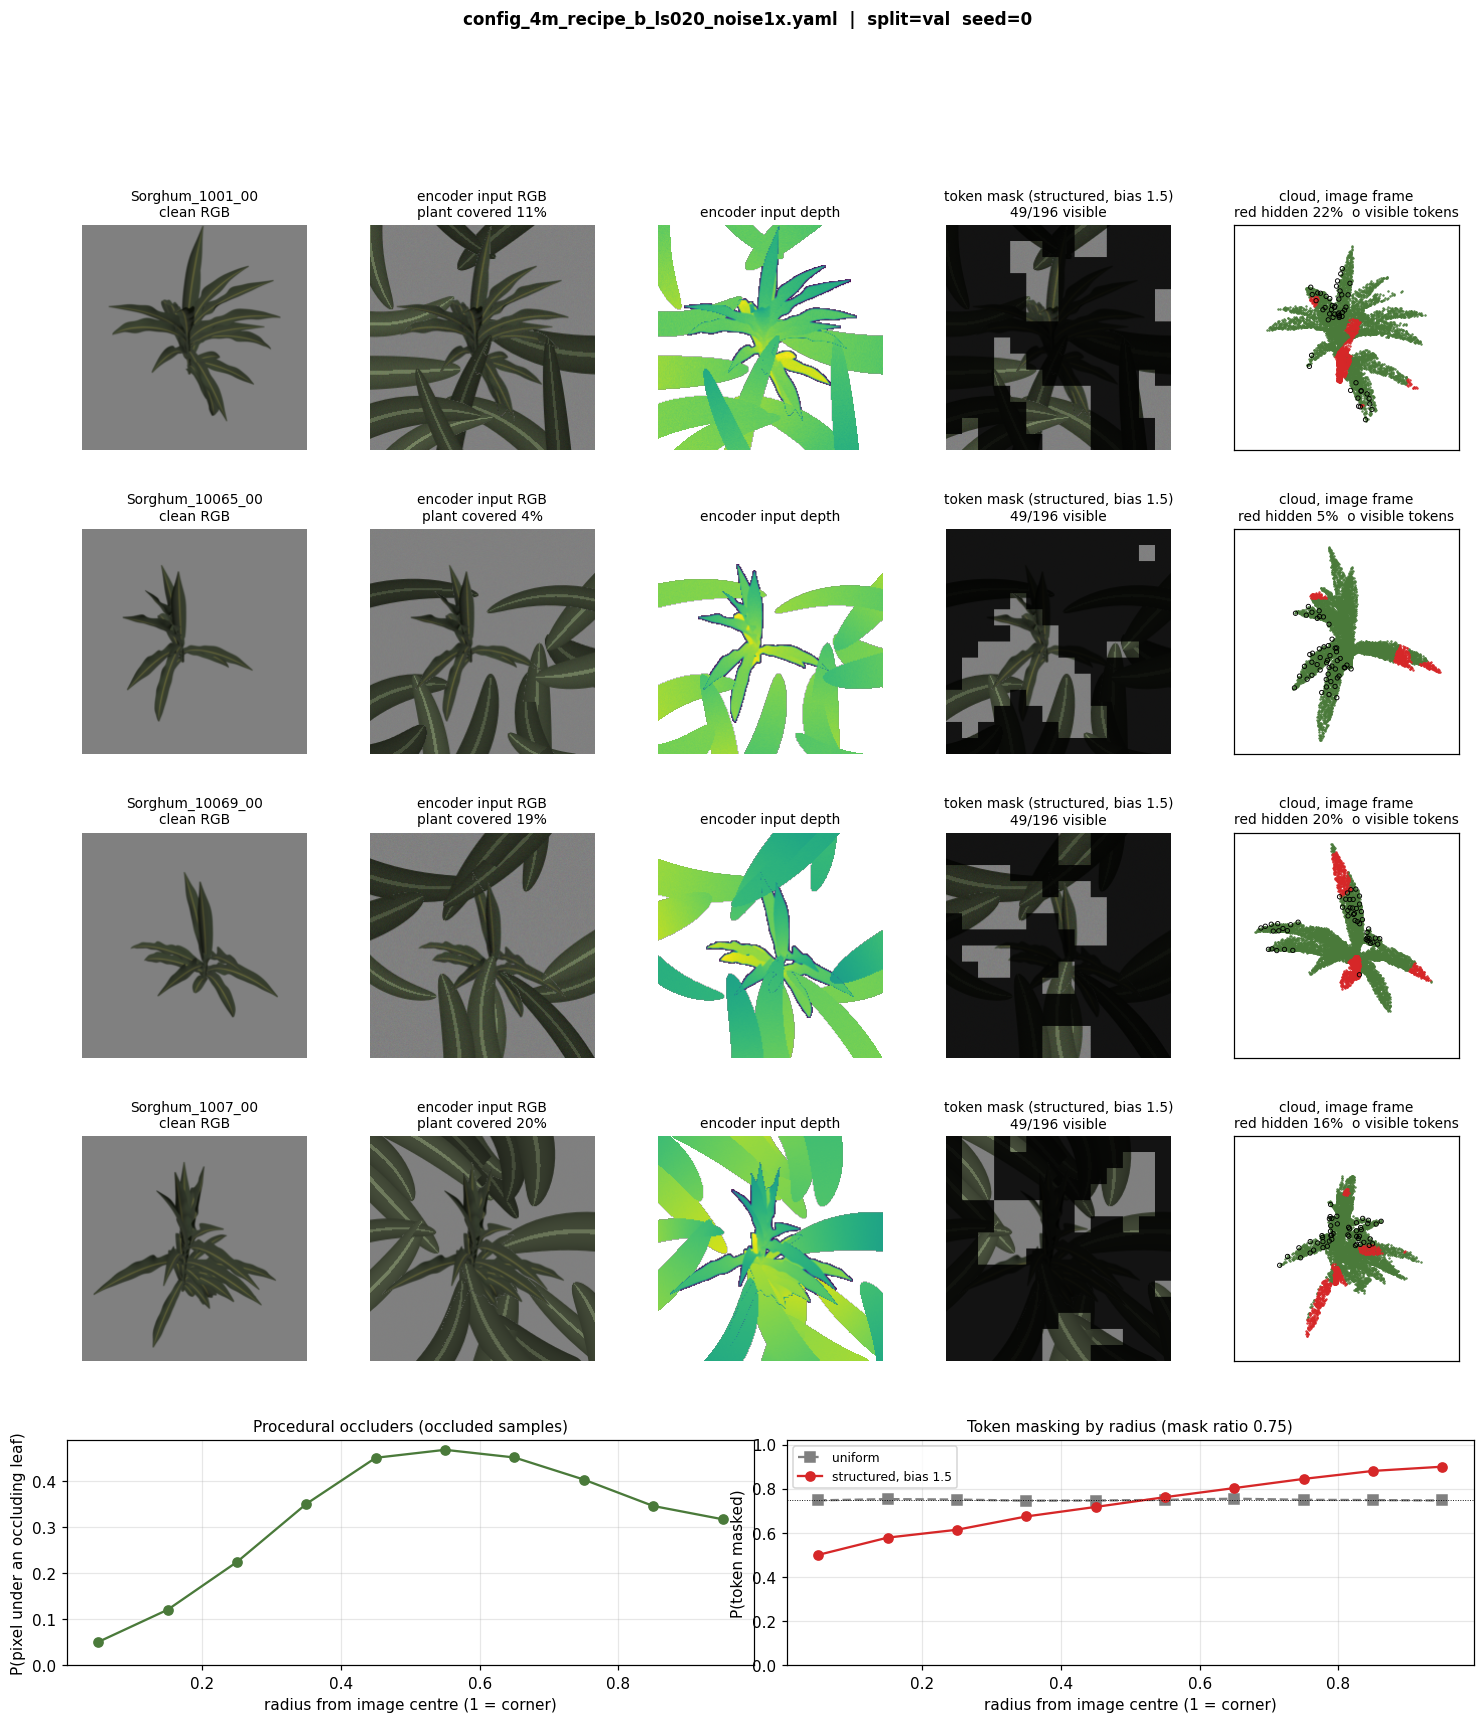
\includegraphics[width=0.92\linewidth,height=\textheight,keepaspectratio]{mask_preview_recipe_b.png}

\textbf{Sensor noise} (added on top of the leaves, to the encoder input
only --- the loss always compares against the clean target). Strength is
drawn per sample and per modality, uniformly between 0 and the maximum
below.

{\def\LTcaptype{none} % do not increment counter
\begin{longtable}[]{@{}
  >{\raggedright\arraybackslash}p{(\linewidth - 6\tabcolsep) * \real{0.2500}}
  >{\raggedright\arraybackslash}p{(\linewidth - 6\tabcolsep) * \real{0.2500}}
  >{\raggedright\arraybackslash}p{(\linewidth - 6\tabcolsep) * \real{0.2500}}
  >{\raggedright\arraybackslash}p{(\linewidth - 6\tabcolsep) * \real{0.2500}}@{}}
\toprule\noalign{}
\begin{minipage}[b]{\linewidth}\raggedright
modality
\end{minipage} & \begin{minipage}[b]{\linewidth}\raggedright
noise
\end{minipage} & \begin{minipage}[b]{\linewidth}\raggedright
max at 1×
\end{minipage} & \begin{minipage}[b]{\linewidth}\raggedright
applied to
\end{minipage} \\
\midrule\noalign{}
\endhead
\bottomrule\noalign{}
\endlastfoot
RGB & additive Gaussian per pixel and channel & ±0.03 (about ±8 of 255
grey levels) & every pixel \\
depth & multiplicative Gaussian & ±1.5 \% of the depth & plant pixels
only (background stays 0) \\
point cloud (\textbf{PC jitter}) & additive Gaussian on x, y and z of
every point & ±0.008 of the unit-radius cloud (about 8 mm on a
\textasciitilde1 m plant) & every point \\
\end{longtable}
}

\textbf{Why jitter the point cloud.}

\begin{itemize}
\tightlist
\item
  \emph{Real 3D sensors are noisy.} The synthetic cloud is sampled from
  the mesh, so every point lies exactly on the surface; depth cameras,
  LiDAR and photogrammetry scatter points in front of and behind the
  surface, most of all on thin leaves. Jitter trains on the kind of
  cloud a real sensor returns.
\item
  \emph{No copying.} Without it, the visible point-cloud tokens already
  contain exact target points and the model can lower the loss by
  reproducing them. With noisy input and a clean target, it has to infer
  where the true surface is --- for example that a leaf which looks like
  a thick layer in the input is a thin sheet.
\item
  \emph{No modality shortcut.} If RGB and depth were noisy but the cloud
  clean, the model could rely on the cloud alone; corrupting all three
  prevents that.
\end{itemize}

At 2× the jitter (about 16 mm) exceeds the F1@0.01 threshold (about 10
mm), so a model must remove it to score. Within 0.5×--2× it made no
measurable difference (section 2), so it is best read as insurance for
real sensor data rather than as a performance lever.

\textbf{Which runs used the corruption} (leaves + sensor noise,
\texttt{prob} 1.0 = every training sample):

{\def\LTcaptype{none} % do not increment counter
\begin{longtable}[]{@{}
  >{\raggedright\arraybackslash}p{(\linewidth - 4\tabcolsep) * \real{0.3333}}
  >{\raggedright\arraybackslash}p{(\linewidth - 4\tabcolsep) * \real{0.3333}}
  >{\raggedright\arraybackslash}p{(\linewidth - 4\tabcolsep) * \real{0.3333}}@{}}
\toprule\noalign{}
\begin{minipage}[b]{\linewidth}\raggedright
runs
\end{minipage} & \begin{minipage}[b]{\linewidth}\raggedright
leaves
\end{minipage} & \begin{minipage}[b]{\linewidth}\raggedright
PC jitter max
\end{minipage} \\
\midrule\noalign{}
\endhead
\bottomrule\noalign{}
\endlastfoot
all 600-epoch runs in sections 1, 3, 5 (including \texttt{maskoff}) and
the main 10k model & on & 0.008 (1×) \\
30k screening, section 2 rows 1, 2, 5 and section 4 & on & 0.008 (1×) \\
30k screening, 0.5× / 2× rows & on & 0.004 / 0.016 \\
original configs (\texttt{config\_4m.yaml}), and main-branch runs built
on them & \textbf{off} & \textbf{none} \\
\end{longtable}
}

Every comparison in this brief therefore holds the corruption fixed.
Rows from runs trained without it (e.g.~the main-branch E1--E4 runs, if
built on the original config) differ in this respect and need a note
when placed in the same table. Validation is completely clean (no
corruption); robustness to corruption is tested separately, on the test
split.

\end{document}
